%! Author = arqfa
%! Date = 8/8/2023

% Preamble
%\documentclass[11pt]{article}
\documentclass[final,5p,times]{elsarticle}
% Packages
%% The amssymb package provides various useful mathematical symbols
\usepackage{amssymb}
%% The amsthm package provides extended theorem environments
\usepackage{amsthm}
\usepackage{graphicx}
\usepackage{tabularx}
\usepackage{booktabs}
%% The lineno packages adds line numbers. Start line numbering with
%%\begin{linenumbers}, end it with \end{linenumbers}. Or switch it on
%% for the whole article with \linenumbers
\usepackage{lineno}
\modulolinenumbers[10]
\usepackage{enumitem}

\usepackage{multirow}

\usepackage{caption}

\journal{Computer Aid Design}


% Document
\begin{document}

\begin{frontmatter}


\title{Embracing Complexity: Mixed Reality Assessment of User Tolerance for Complex Facades in Future Construction Trends}

%% use optional labels to link authors explicitly to addresses:
%% \author[label1,label2]{}
%% \affiliation[label1]{organization={},
%%             addressline={},
%%             city={},
%%             postcode={},
%%             state={},
%%             country={}}
%%
%% \affiliation[label2]{organization={},
%%             addressline={},
%%             city={},
%%             postcode={},
%%             state={},
%%             country={}}

\author[inst1]{Fabian Jarrin}
\author[inst1]{Yasuko Koga}
\author[inst2]{Diego Thomas}

\affiliation[inst1]{organization={Graduate School of Human-Environment Studies, Department of Architecture and Urban Design, Kyushu University},%Department and Organization
            addressline={744 Motooka, Nishi Ward},
            city={Fukuoka},
            postcode={819-0382},
            state={Kyushu},
            country={Japan}}

\affiliation[inst2]{organization={Graduate School of Information Science and Electrical Engineering, Kyushu University},%Department and Organization
            addressline={744 Motooka, Nishi Ward},
            city={Fukuoka},
            postcode={819-0382},
            state={Kyushu},
            country={Japan}}

\begin{abstract}
%% Text of abstract
This research aims to evaluate the efficacy of virtual reality (VR) simulations in promoting the acceptance of data-driven optimized design solutions for Site Layout Planning (SLP). The study involves the development of a multi-objective optimization model, considering essential factors such as earthwork volume calculations, cost, and environmental impact, particularly for an educational building located on the site. The model is subsequently transformed into an interactive VR simulation, enabling participants to visually observe the real-time impact of various building placements on the site. The results indicate that the utilization of the VR simulation significantly enhances the understanding and acceptance of the recommended data-driven optimized design solutions. On average, participants experienced a notable \(48.3\%\) increase in accuracy compared to traditional methods. The technology was highly regarded by participants, receiving an average acceptance rate of 5.4 on a 7-point Likert scale. It is essential to recognize that while VR simulations show promise in expediting the adoption of data-driven optimized design solutions, they are not intended to replace existing design review methods. Instead, they serve as a means to streamline the decision-making process and provide stakeholders with a more immersive and comprehensive understanding of the design solutions.

        %This research focuses on assessing the effectiveness of virtual reality (VR) simulations in promoting the acceptance of data-driven optimized design solutions for Site Layout Planning (SLP). To achieve this, a multi-objective optimization model was developed, taking into account important factors such as earthwork volume calculations, cost, and environmental impact, particularly for an educational building situated on the site. The model was then transformed into an interactive VR simulation, allowing participants to visually observe the real-time consequences of different building placements on the site. 
        %The findings of the research indicate that the utilization of the VR simulation significantly enhanced the understanding and acceptance of the recommended data-driven optimized design solutions. On average, participants experienced a notable \(48.3\%\) increase in accuracy when compared to traditional methods. The technology itself was highly regarded by participants, receiving an average acceptance rate of 5.4, across several levels, on a 7-point Likert scale.
        %It is important to note that while VR simulations show promise in expediting the adoption of data-driven optimized design solutions, they are not meant to replace existing design review methods. Instead, they serve as a means to streamline the decision-making process and provide stakeholders with a more immersive and comprehensive understanding of the design solutions.
        


\end{abstract}


%%Graphical abstract

\begin{graphicalabstract}
    \centering
    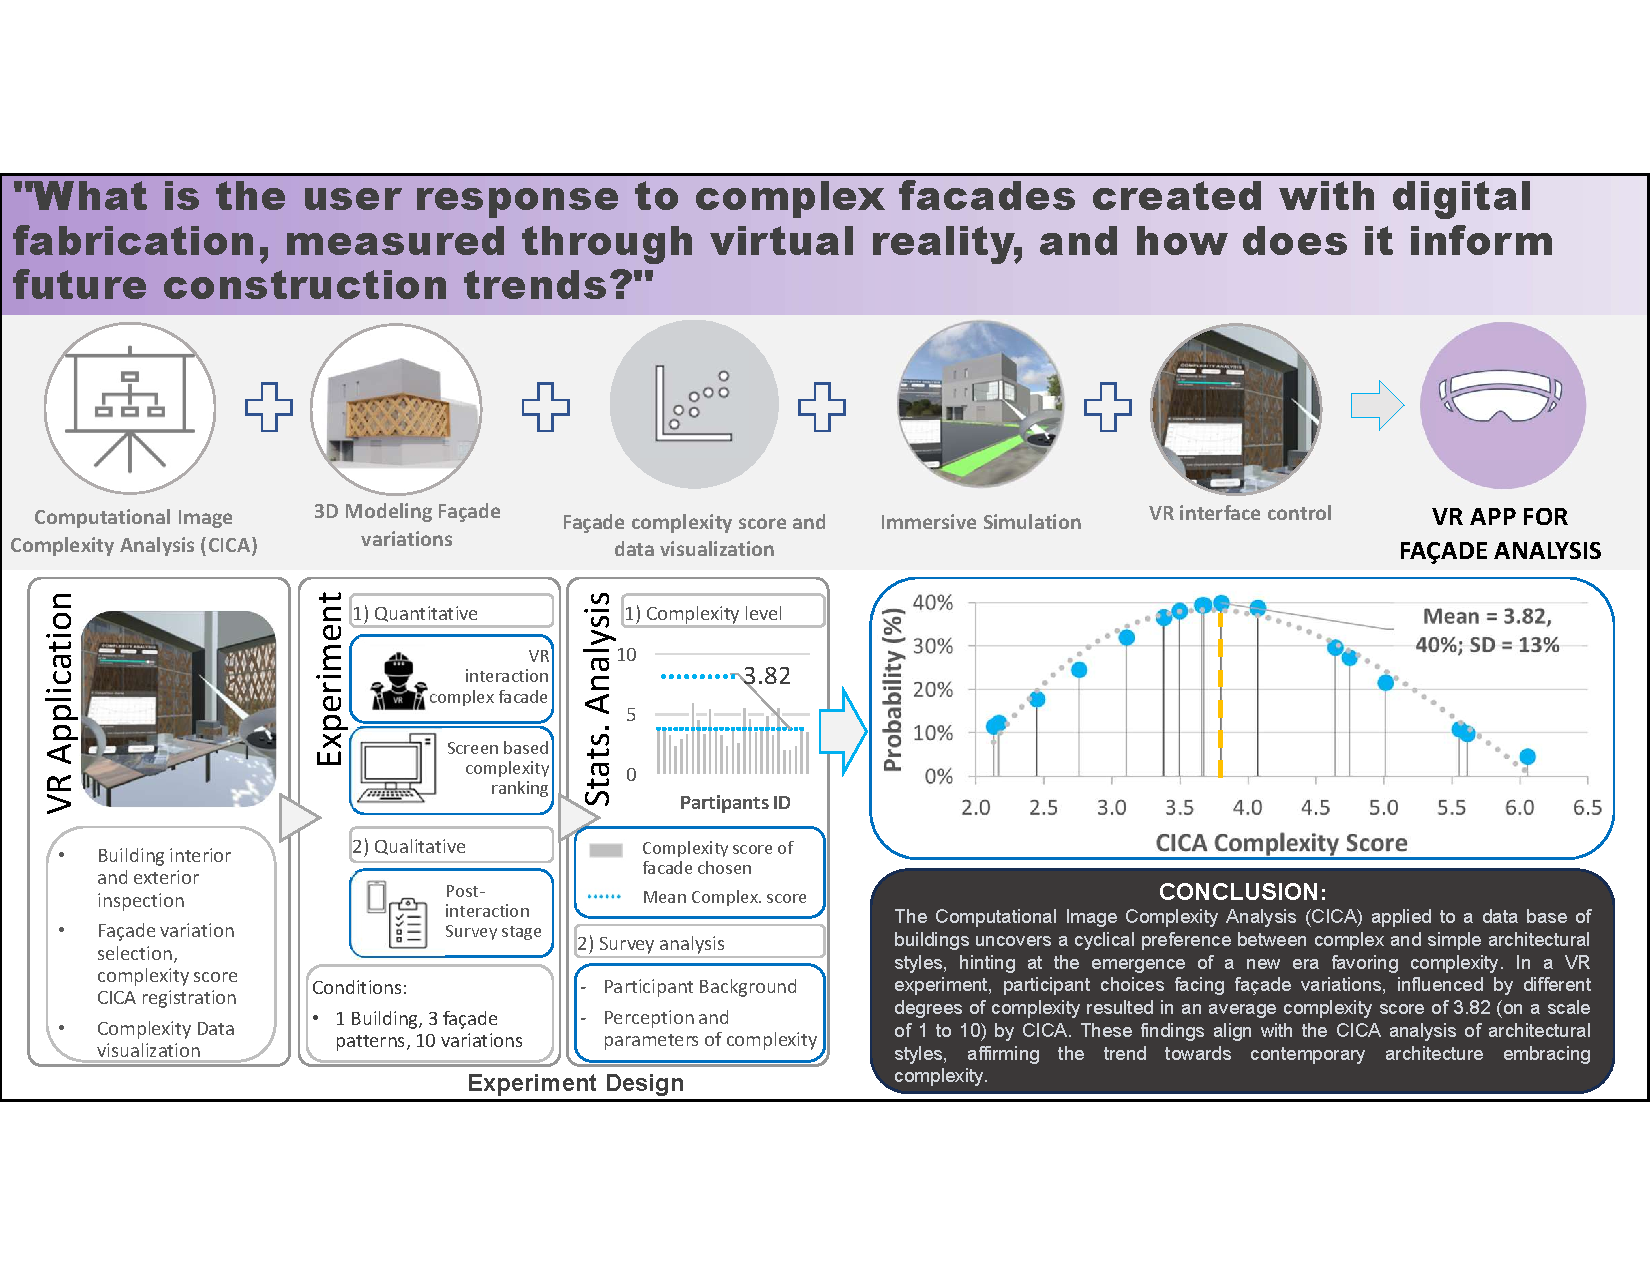
\includegraphics[width= \textwidth, trim = 0 80 0 80, clip]{Images/GraphicAbstract.pdf}
    \label{fig:graphic_abstract}
\end{graphicalabstract}

%%Research highlights
\begin{highlights}
%highlights

\item Computational Image Complexity Analysis (CICA) system using computer vision.
\item CICA system quantifies facade complexity, aiding in historical trend analysis.
\item VR experiment indicates user preference for moderate complexity in facades.
\item Future architecture favoring user-centric, complexity balanced designs trends.

\end{highlights}

\begin{keyword}
%% keywords here, in the form: keyword \sep keyword
Data-driven design\sep Site Layout Planning \sep Virtual reality \sep Optimization\sep

\end{keyword}

\end{frontmatter}
%\linenumbers
%\modulolinenumbers[10]
%
\begin{linenumbers}


\section{Introduction}
\label{sec:1Introduction}
%%State the objectives of the work and provide an adequate background, avoiding a detailed literature survey or a summary of the results.
%%Introduction

%=================================
%%Reference
%%https://www.scribbr.com/research-paper/research-paper-introduction/
%%State the objectives of the work and provide an adequate background, avoiding a detailed literature survey or a summary of the results.

%Step1. Introduce your topic.
     %This is generally accomplished with a strong opening hook.
%Step2. Describe the background.
     %For a paper describing original research, you’ll instead provide an overview of the most relevant research that has already been conducted.
%Step3. Establish your research problem.
     %In an empirical research paper, try to lead into the problem on the basis of your discussion of the literature.
%Step4. Specify your objective(s).
     %The research question is the question you want to answer in an empirical research paper. If your research involved testing hypotheses, these should be stated along with your research question.
%Step 5: Map out your paper.
     %The final part of the introduction is often dedicated to a brief overview of the rest of the paper.

%recommended limit 500 words
%=================================

Recent advancements in Building Information Modeling (BIM) and digital fabrication are transforming architectural practice.
These technologies enable architects to design intricate and complex forms, moving beyond the uniformity of barren walls and fully glazed facades that often dominate contemporary streetscapes.
By leveraging these advancements, architects can introduce complexity and detail into their designs, enhancing both the visual and functional aspects of buildings, and creating more engaging and dynamic environments that potentially redefine the relationship between form and function~\cite{Leach2016}.

However, the pursuit of complexity in architectural design must be balanced with sustainability and user satisfaction.
Designs that are overly complex without consideration of these factors can quickly become outdated and disconnected from their inhabitants, leading to issues of obsolescence and lack of relevance~\cite{Oberfrancova2021}.
Understanding how complexity can enhance both environmental sustainability and user satisfaction is therefore crucial for modern architectural practice.

Previous research has extensively explored the impact of complexity in architectural design, identifying mathematical relationships between complexity and aesthetic value ~\cite{Bies2016, Douchova2016, Redies2015}.
Despite these insights, the architectural field has yet to develop frameworks that leverage these principles for practical design applications, especially considering modern technological advancements aimed at sustainability.

This study aims to bridge the gap between theoretical understanding and practical application by developing a methodology to measure facade complexity.
The objectives are to generate data that can improve `Data-driven Building Design' (DBD) by integrating a complexity scoring function that can inform on the optimal rate between simplicity and complexity based on historical analysis and user preferences.
By integrating complexity insights with modern technological applications, we seek to provide actionable, DBD insights for future architectural practices promoting the advancement aimed at sustainability.

The methodology is structured around 4 primary components:

\begin{enumerate}
    \item Literature review: Significant studies on the foundational theories of complexity, and an exploration of the fluctuation between simplicity and complexity in architectural history.
    \item Complexity Analysis System Development: Implements a Virtual Reality (VR) framework, and combines it with a Computational Image Complexity Analysis (CICA) component using computer vision (CV) algorithms to quantitatively assess the complexity of facade designs.
    \item Experiment Execution: involving VR to facilitate participant interaction with complex facades, augmented by surveys and interviews for qualitative insight.
    \item Data Analysis and Validation: Assessing the data collected during the experiment to evaluate the effectiveness of the Complexity Analysis System and CICA framework in measuring complexity and user preferences.
\end{enumerate}

\deleted{This comprehensive approach aims to enrich our understanding of facade complexity and its role in the contemporary Architectural, Engineering, and Construction (AEC) industry.}

This comprehensive approach aims to enrich our understanding of facade complexity and its role in the contemporary Architectural, Engineering, and Construction (AEC) industry.

\added{Comment 1: The author emphasized the importance of integrating sustainability and user satisfaction into facade design. However, how this study addresses sustainability concerns is not explicitly stated. Therefore, please provide further clarification on this aspect.}



%
%!Notes
Beauty is too difficult to translate into number so why bother?
Is beauty really subjective?
Why would we care? there is an

A 2011 survey in the United States found the strongest correlation between a place's physical beauty, and peoples satisfaction out of any other attributes!

Design disconnect. Architects and the public each seem to like different kinds of buildings. This effect was discovered by psychologist David Halpern. Study in 1987.

Beauty is nature way of

According to Denis Dutton, all things that we find beautiful have three things in common: Firstly: they have a shape or characteristics we inherently like.
Secondly, they are fit for their purpose.
And thirdly, they are well-made and display skill in their making.

Organised complexity. As humans, we seem to need some complexity or diversity of form but not too much. Only order is boring, but only complexity is chaos. We seem to like things that are somewhere in the middle. A plain facade too ordered, so we ignore it. A facade like this on the other hand is too

Evidence based design

%!Sustainability
%cause gimmicks, like fashion, get outdated at some point. Many buildings built in the last 50 years already need to be torn down, as they did not have the qualities that made people connect to them. All this renovating and rebuilding requires massive amounts of new concrete, glass and steel. All at a huge cost for society. And, of course, for the environment.


%!Thesis
%we link fractals and organized complexity to environmental optimization to combine them in a theory od data driven beauty environental design. We established that the complexity theory and the vr influence as representative of MR tehconologies serves to built on the aspect of creating a paneling system with organized complexity since it has proven that beauty is perceived by it and we guarantee to add value and improtance to cities based on the papers and video "What makes a building beuatiful".
%!Video article

Architecture:\cite{Aesthetic2022}



Organise your facade in a clear, readable way, so people can make sense of how load bearing features connect to each other
Apply some form of ornament to connect separate parts of the building and to offer the fractal & symmetrical qualities people subconsciously connect to
Prevent the creation of large blank walls or glass facades at eye level. Glass is hard to ‘read’ – people can’t focus their eyes well on it as it is partly reflective, partly translucent.
Apply (local) symmetry in your design. The building can be asymmetrical if building volumes on both sides of a central axis are ‘balanced’
Richly detail the facade if possible, with details on various levels of scale, or utilise materials with some pattern to offer fractal qualities in the surface
Build according to local preferences, history, culture – study the ‘Genius Loci’.
Use curves in your design wherever possible
Urbanism:

Utilise street trees wherever possible
Apply ‘gentle density’: “In contrast to high density, which includes mid- and high-rise residential buildings, gentle density refers to development of duplexes, triplexes, accessory dwelling units (ADUs), stacked townhouses, semi-detached homes and small-scale apartment and condominium buildings within and among single-family zoned neighborhoods. Gentle density promotes mixed-use development, with single-family homes alongside small multi-family homes, businesses and commercial buildings. Gentle density aims to retain neighborhoods’ residential identity and feel while alleviating housing crises.”

modern brain imaging methods have empowered studies on how aesthetic experience
correlates with the activation of brain regions in the human
observer and advanced computational methods permit the investigation of statistical
image properties that are associated with aesthetically pleasing images\cite{Redies2015}

Despite the uncertainties, there seems to be a general agreement in the field that the scien-tific study of aesthetic experience and of beautiful stimuli holds
great promise and may contribute significantly to our under-
standing of human brain function and behavior\cite{Redies2015}

Birkhoff (1933)\cite{Birkhoff1933} first formalized aesthetic value as the ratio of order and complexity.
Complexity, to Birkhoff (1933), was a
physical, measurable characteristic that could be described
mathematically \cite{Bies2016}

Birkhoff\cite{Birkhoff1933} defines an aesthetic measure and applies it to several types of objects with different modes of perception – visual, including
3D objects, and auditory (music, poetry).
The measure is defined in relation to the effort which the object demands of the perceiver (complexity), and the pleasing or displeasing features which can be recognised in the object (order).\cite{Douchova2016}
%!aesthetics

Recent experimental studies began examining the neuroaesthetics of the built envi-
ronment [166–170]. But most offer a perspective almost completely limited to modernist
aesthetics and fail to consider traditional design let alone the fractal mathematics of per-
ception [3,171–180]. \cite{Brielmann2022}

%!Complexity

Complexity & Order is rich sensory information that adheres to a spatial hierarchy similar to those encountered in nature. \cite{Browning2014}

A space with good Complexity & Order feels engaging and information-rich, as an intriguing balance between boring and overwhelming.\cite{Browning2014}

The Complexity & Order pattern has evolved from research on fractal geometries and preferred views; the perceptual and physiological responses to the complexity of fractals in nature, art and architecture; and the predictability of the occurrence of design flows and patterns in nature.\cite{Browning2014}




Researches have found that
The consistency of natural themes in historic structures and places suggests that
biophilic design is not a new phenomenon; rather, as a field of applied science,
it is the codification of history, human intuition and neural sciences showing that
connections with nature are vital to maintaining a healthful and vibrant existence
as an urban species.\cite{Browning2014}

Fractals are patterns that repeat at increasingly fine sizes and so create shapes of rich visual complexity.
Prevalent in nature, clouds, trees, and mountains are common examples, as are cauliflowers and fern leaves.
This paper dives into the complex minutiae of vision and fractals, and how they can place the observer in the “comfort zone”.\cite{Browning2014}

Richly detail the facade if possible, with details on various levels of scale, or utilise materials with some pattern to offer fractal qualities in the surface\cite{Aesthetic2022}

Complexity & Order is rich sensory information that adheres to a spatial hierarchy similar to those encountered in nature. \cite{Browning2014}

A space with good Complexity & Order feels engaging and information-rich, as an intriguing balance between boring and overwhelming.\cite{Browning2014}

The Complexity & Order pattern has evolved from research on fractal geometries and preferred views; the perceptual and physiological responses to the complexity of fractals in nature, art and architecture; and the predictability of the occurrence of design flows and patterns in nature.\cite{Browning2014}

Birkhoff (1933)\cite{Birkhoff1933} first formalized aesthetic value as the ratio of order and complexity.
Complexity, to Birkhoff (1933), was a
physical, measurable characteristic that could be described
mathematically \cite{Bies2016}

Birkhoff\cite{Birkhoff1933} defines an aesthetic measure and applies it to several types of objects with different modes of perception – visual, including
3D objects, and auditory (music, poetry).
The measure is defined in relation to the effort which the object demands of the perceiver (complexity), and the pleasing or displeasing features which can be recognised in the object (order).\cite{Douchova2016}




Traditional architecture knew how to explore \cite{Browning2014}



Despite extensive research in data-driven building design aimed at optimizing resource use and environmental sustainability, many buildings still fail to resonate with the people who inhabit them, leading to premature demolition.
Computational advancements have the potential to transform urban landscapes; however, without addressing the psychological connection between people and their built environment, even sustainably designed buildings may suffer the same fate as their predecessors, cause fashion-like gimmicks become obsolete over time, leading to significant societal and environmental costs\cite{Aesthetic2022}.
Beauty significantly contributes to emotional attachment and happiness in urban areas\cite{Brielmann2022}, yet beauty is largely considered as subjective and relinquished to aesthetic ideologies generating short-fashion urban fabric, however neuroscientists and anthropologists have found certain universal preferences organized in built structures on neurophysiological criteria and measurements that allow to circunvent old and inconclusive debates in aesthetics and architectural history\cite{Brielmann2022}.

Citations by brielmann 2022

The data reviewed here show that we fundamentally need to change how we design
the built environment.
It is time for people to place urban well-being above aesthetic ideology; the durability and long-term reusability of urban fabric above fashion. Changing
built environments—from “old-fashioned” to new, slick, and shiny—is a huge mistake, as people all over the world realize that we need emotional nourishment from the environment around us.
“Old-fashioned” surroundings could likely contain essential healing qualities.
We deserve to walk down a street that is beautiful, as judged by our biology, not by
some imposed stylistic criterion.
We deserve to be protected from the negative psychological reactions caused by experiencing neuroaesthetically inappropriate if not harmful design.
Based on our latest scientific understanding of perception, we need to reclaim
the appropriate and practical design toolkits of past generations to accomplish these ends.
Only then will we be able to build places for the greatest well-being of the greatest number of users.


Yet a new issue arises while extensive research in data-driven building design has been done in pursuit of optimization of resources and environmental engineering, buildings continue to fall out of grace and being demolished by failing to connect with the people that inhabit them.
The computational advancements provide the chance to transform the city scape however if no attention is directed to bring about that attachment with people regardless of it sustainability these new buildings will follow the same lifespan as their predecessors, cause gimmicks like fashion, get outdated at some point All at a huge cost for society. And, of course, for the environment. \cite{Brielmann2022}



\section{Research Background}
\label{sec:Background}
%% A Theory section should extend, not repeat, the background to the article already dealt with in the Introduction and lay the foundation for further work. In contrast, a Calculation section represents a practical development from a theoretical basis.
%% Research Background

%% A Theory section should extend, not repeat, the background to the article already dealt with in the Introduction and lay the foundation for further work. In contrast, a Calculation section represents a practical development from a theoretical basis.

\subsection{Timeline of Architecture styles}
\label{subsec:TimelineArchitectureStyles}
We evidence this when observing the Romanesque classical style on the 10 th century found mostly in churches ith thick wall structures, followed by the breakthrough in load distribution during the Gothic style of the 12th to the 16th century which abandons the robustness to erect high buildings with complex great stained windows.
The Renaissance follows at the end of the middle ages and with it the return of the classical order with round arch and classical order columns that brings ornaments back to the interior in favour of more simplified exteriors. In reaction to this style Baroque style surges with more dynamic forms , irregular shapes and exagerated ornamentation in bold combinations.

%%%%


\end{linenumbers}
    \bibliography{main}
    %\bibliographystyle{plain}
    \bibliographystyle{elsarticle-num}

\end{document}